\section{Introduction}

Language-model internals have been associated with feed-forward memories,
knowledge neurons, and causally important states
\citep{geva-etal-2021-transformer,dai-etal-2022-knowledge,
NEURIPS2022_6f1d43d5}. This literature suggests an operational hypothesis:
once information is localized, the corresponding representation should provide
a useful control point. Activation steering tests that hypothesis without changing model parameters
\citep{turner2023steering,rimsky-etal-2024-steering,zou2023representation,
pmlr-v235-singh24d}. Yet behavior varies across prompts, layers, models, and
coefficients, and stronger interventions can damage specificity or unrelated
capabilities \citep{NEURIPS2023_81b83900,stoehr-etal-2024-activation,
tan2024steering,goyal-iii-2026-steering}. Steering is thus a multidimensional
control problem \citep{wu25a,pres2024reliable,xu-etal-2026-controllable}.

Localization describes a representation, whereas controllability is revealed
across a \emph{measured intervention path}. Target leverage can coexist with
semantic-neighbor or capability damage, and a clean effect at one coefficient
need not persist at another. Predicting calibrated target, damage, and clean
outcomes over a pre-specified grid asks which localized directions admit a
usable measured coefficient. A single endpoint cannot answer this question:
the same direction may show leverage at one measured strength, damage at
another, or no coefficient where the two separate cleanly.

We introduce \emph{Predictive Memory Localization} (PML), which maps each
record, direction, and layer to those random-calibrated outcomes. It organizes
predictive evidence from baseline belief and metadata, static localization, and
supervised representation geometry to a strength-disjoint low-dose causal
response. This design directly tests whether static evidence forecasts later
behavior or whether an inexpensive causal measurement is required. A
collateral-aware policy then selects a coefficient or abstains.
Unlike generation-level concept prediction \citep{fan2026steerable}, PML audits
localized factual and reasoning directions with explicit collateral probes and
strength-disjoint labels.

\begin{figure*}[t]
    \centering
    \begin{tabular}{@{}c@{\qquad}c@{}}
        \small\textbf{(a) Internal representation} &
        \small\textbf{(b) Forecast utility and decide} \\
        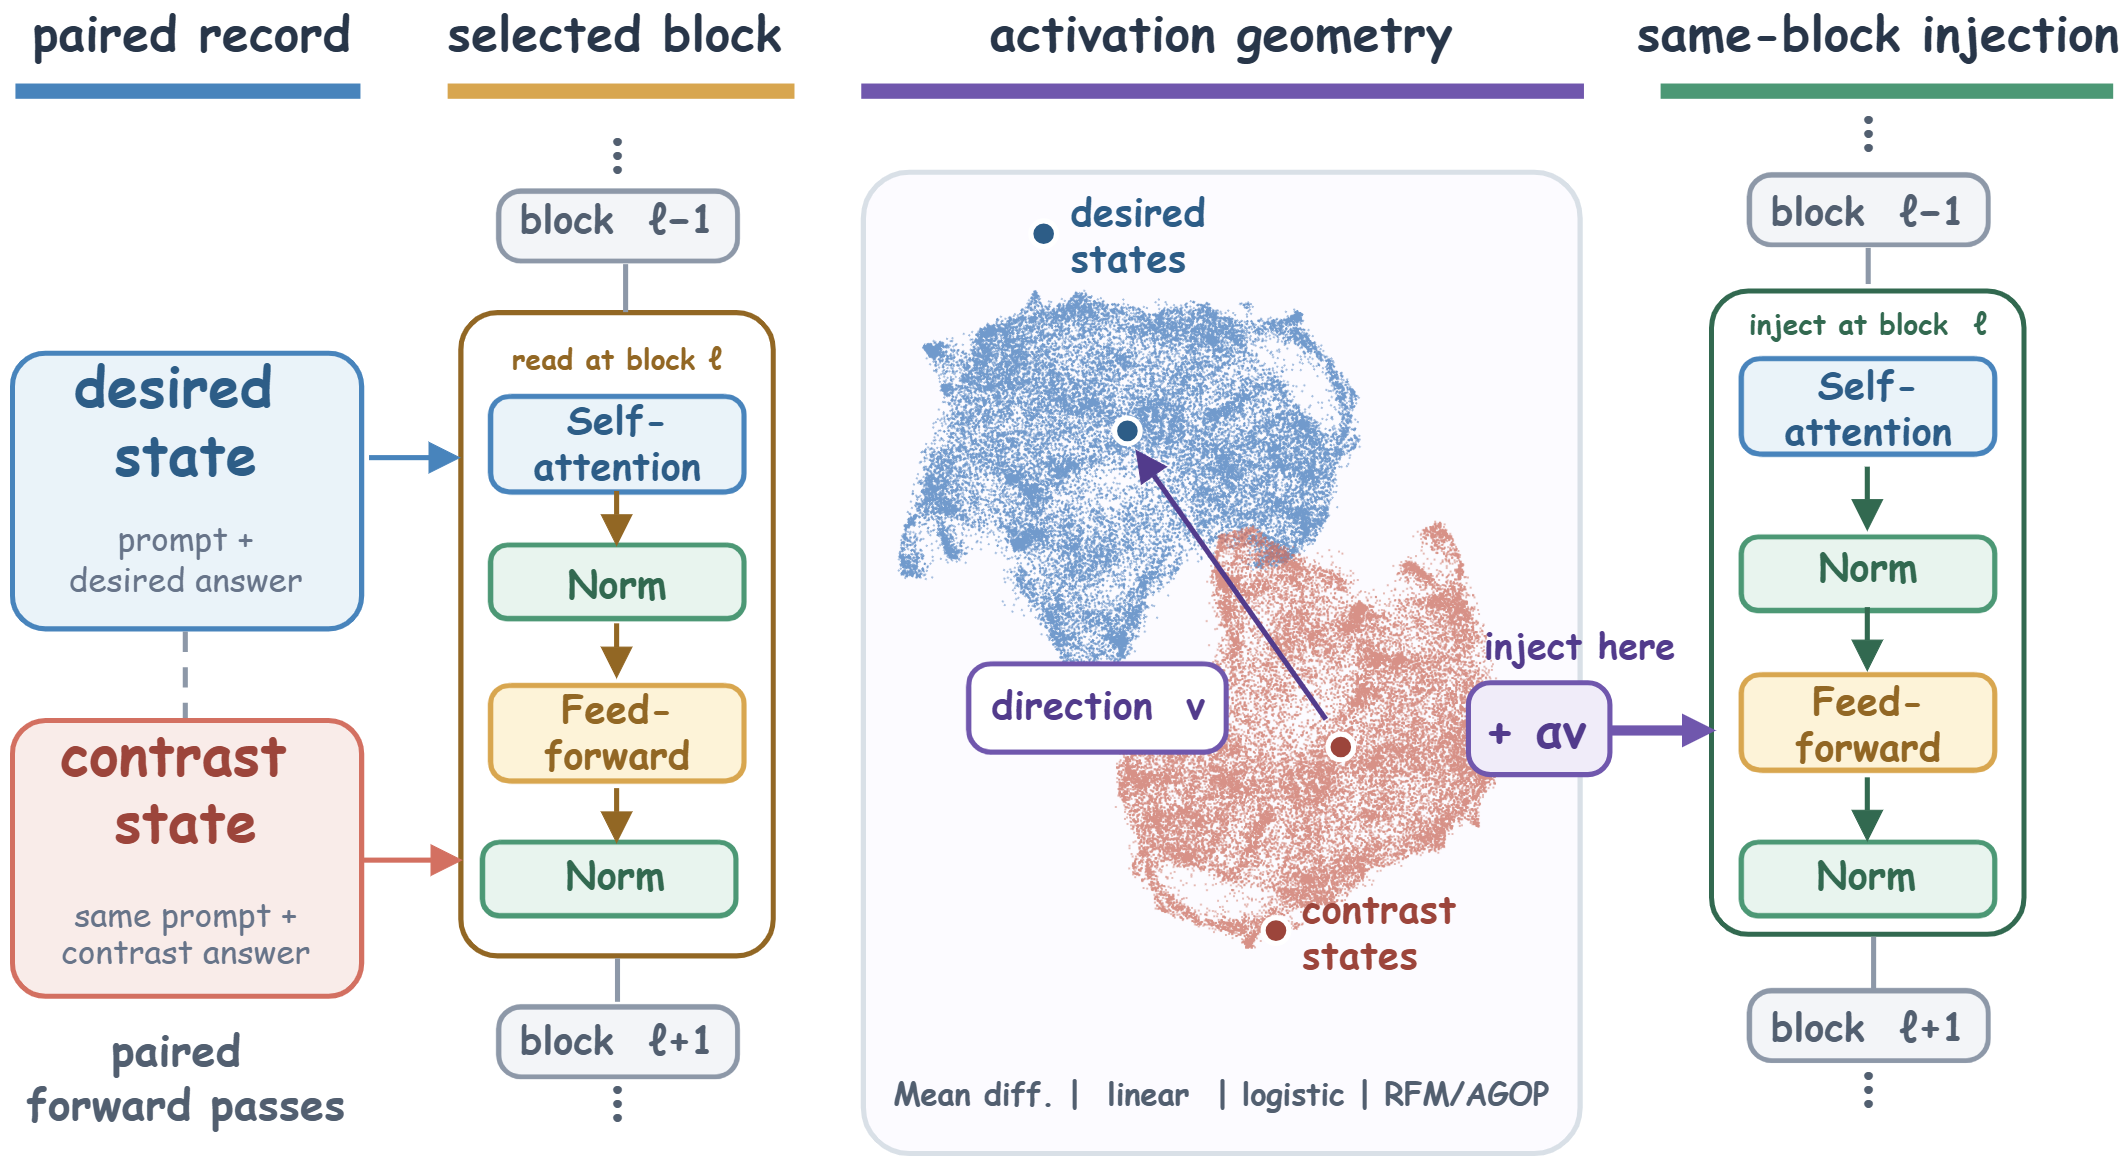
\includegraphics[width=0.45\textwidth,height=2.45in,keepaspectratio]{figures/figure1_internal_representation.png} &
        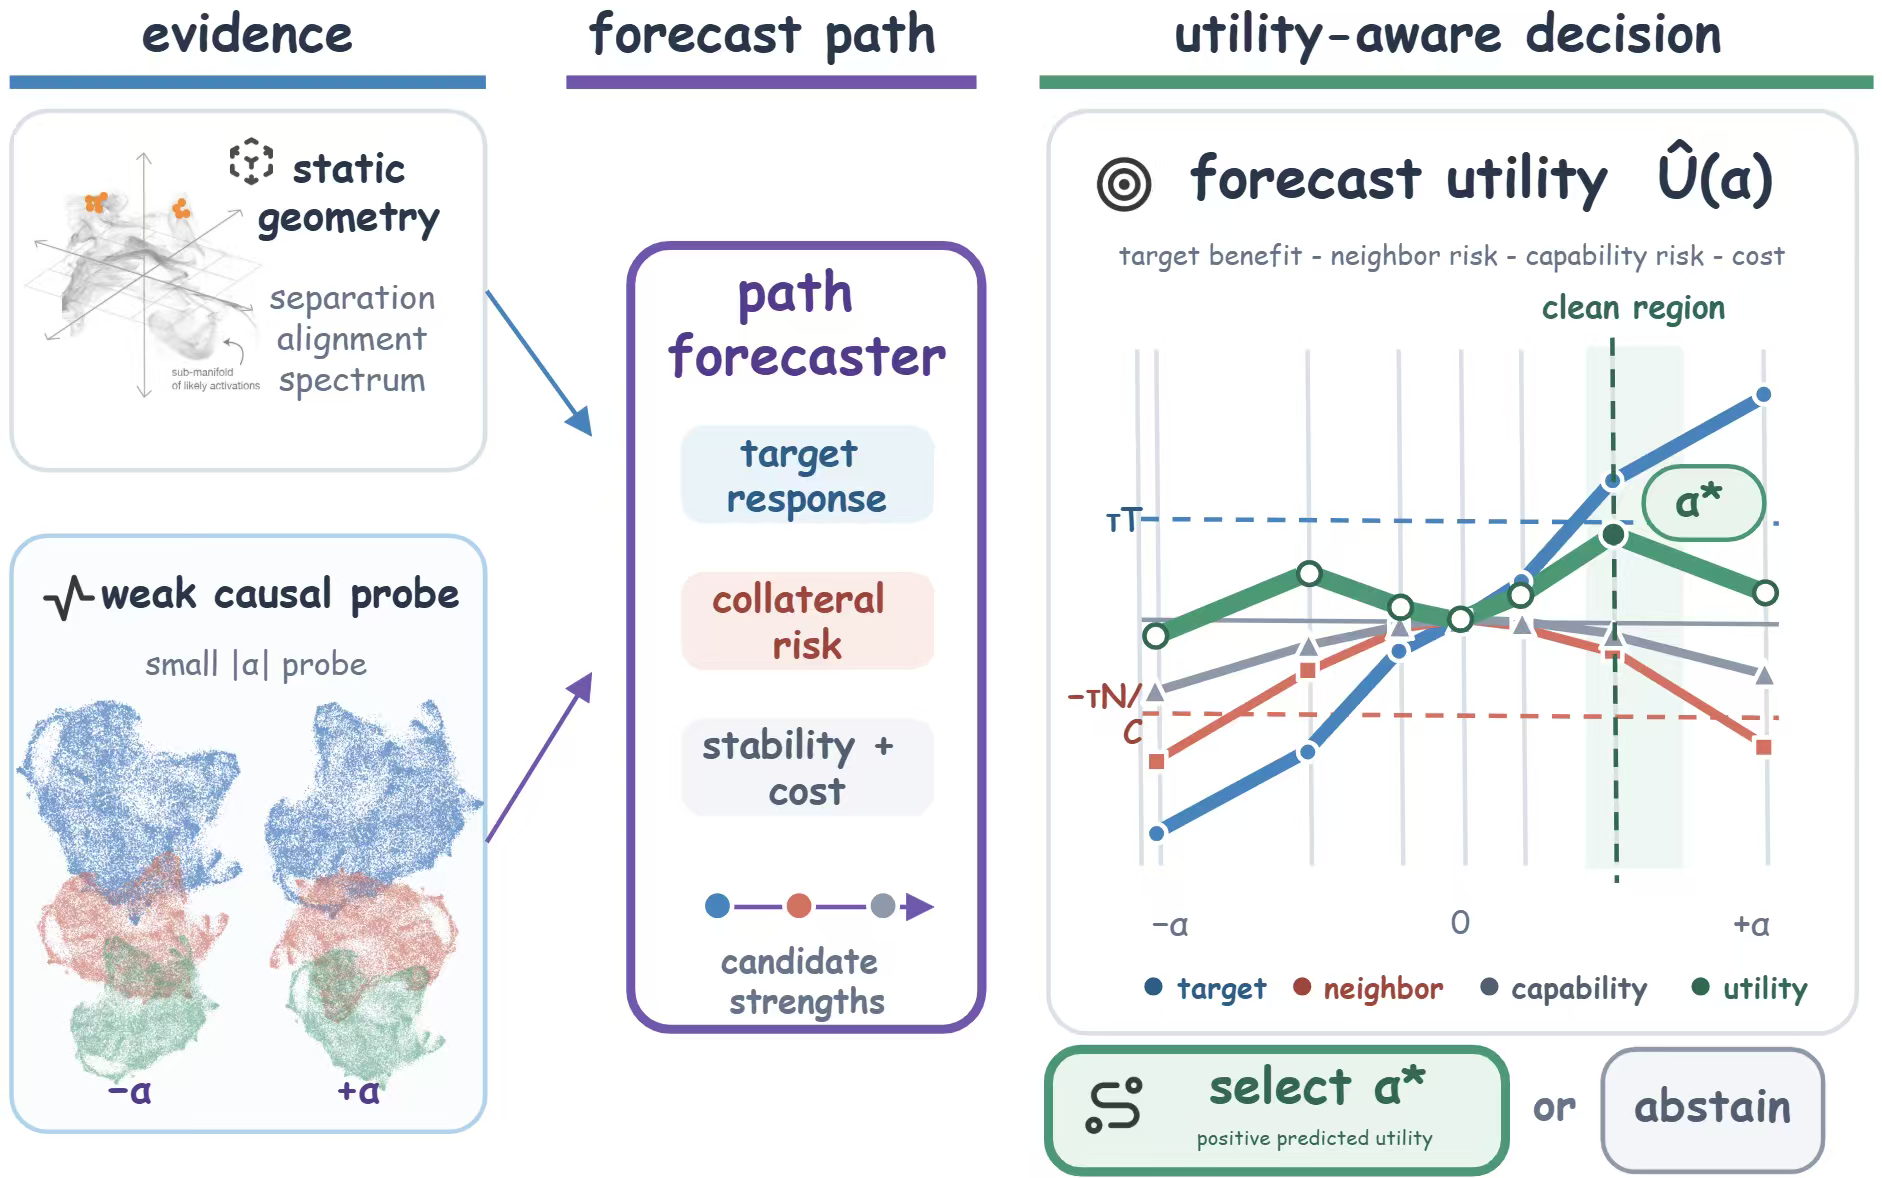
\includegraphics[width=0.45\textwidth,height=2.45in,keepaspectratio]{figures/figure1_forecast_decide.png}
    \end{tabular}
    \caption{PML from representation to selective control. (a) Direction
    estimators use desired and contrast activations at a selected block, where
    the resulting direction is injected. (b) Static evidence and a disjoint
    low-dose response forecast target benefit, collateral risk, and utility
    over candidate coefficients for selection or abstention. Curves are
    schematic.}
    \label{fig:pml-pipeline}
\end{figure*}

On 3,000 frozen records from nine datasets and fourteen domains, learned
directions improve target and clean-path incidence over random. Static
localization adds little predictive value, whereas a disjoint low-dose response
dominates later-path prediction across grouped transfer. Both findings replicate
across three residual-norm-matched base models (0.801--0.828 record-held-out
macro AUROC). A held-out selector improves utility and reduces neighbor damage
relative to a fixed intervention. The central result is that \textbf{a small
causal response is the most useful forecast of later selective behavior.}

This work makes three contributions:
\begin{itemize}
    \item We define a random-calibrated measured-grid path that jointly records
    target leverage, semantic-neighbor damage, capability damage, and clean
    measured coefficients for each record, direction, and layer.
    \item We separate static localization and supervised geometry from a
    strength-disjoint causal probe, showing that the former are weak predictive
    priors while the latter supplies the dominant signal across grouped and
    cross-model evaluation.
    \item We connect forecasting to action with a held-out collateral-aware
    policy that selects one coefficient or abstains, providing a proof of
    concept for reducing dense intervention evaluation.
\end{itemize}
